% # -*- coding: utf-8 -*-
\section{Implementation}\label{subsection:implementation}
% 実現方式の想定環境は,x86\_64 CPUアーキテクチャの Linux とし,権限情報保護を目
% 的とした方式,ならびにカーネルのセキュリティ機能の保護を目的とした方式の2つの
% 実現方式を考案した.
%
% 保護対象カーネルデータとして,権限情報を想定し,システムコール単位で読書き制限
% の管理を動作中のカーネルにて行う実現方式を考案した.実現方式にて想定する環境
% は,x86\_64 CPUアーキテクチャの Linux としている.

In this study, the KDPM is implemented on Linux with the x86\_64 CPU
architecture. 
%
% There are two implementations are as following: 
Table \ref{tb:consideration_implementation} presents the protected kernel data
and write control timing according to the implementations. 
% are shown in  and following:
The following are the implementation details:

%one for protecting authorization information and the
% other for protecting the kernel security functions.

\begin{table}[t]
  \centering
 \caption{
   %  Portability consideration of MKM mechanism for OSes ($\checkmark$ is supported; $\triangle$ is partially supported).
   %実現方式の比較 %($\circ$: covered ; $\bullet$: non-covered;)
   Comparison of the implementations of the KDPM
   }
 %\vspace{-0.5ex}  
 \scalebox{0.9}{
 %  \begin{tabular}{c|cc}
 \begin{tabular}{ccc}    
 %\hline
 \hline
 \noalign{\smallskip}
 %\begin{tabular}{c}
 %  {\bf Feature}
 %\end{tabular}
\begin{tabular}{c}
  {\bf Item}
\end{tabular}
&
\begin{tabular}{c}  
  {\bf Implementation 1} 
\end{tabular}
& 
\begin{tabular}{c}
  {\bf Implementation 2}
\end{tabular}  
  \\
 \noalign{\smallskip}
 \hline
 \noalign{\smallskip}
 Protected kernel data   & Privilege information & Function pointer \& Access policy\\
%  Handling granularity     & System call            & Kernel code \\
 Handling                & System call            & Kernel code \\
 Mitigation              & Privilege escalation  & MAC defeating\\ 
 Performance             & High                   & Low \\
%  Stability effect                & Low          & High \\

 \hline
 \end{tabular}
 }
 \label{tb:consideration_implementation}
 %\vspace{-1.0ex}  
 \end{table}


%\begin{itemize}[topsep=0pt]%\topsep=-1.0ex \itemsep=-1.0ex \parskip=1.0ex
\begin{itemize}
%   \item {\bf 実現方式1}:書込み許可システムコールとして,権限情報の変更を行うシ
%   ステムコールの実行時のみ,権限情報を格納したカーネルデータを書込み可能に制御
\item Implementation 1: This manages the protected kernel data containing
privileged information and write-permitted system calls that change the
privileges of the user process. 
%
Even if a user process attempts a privilege escalation, the privilege
information cannot be written during the execution of another system call.
% , thereby deterring the attack.

% auth information.
%  is executed.
% . to be writable only
 

%   \item {\bf 実現方式2}:書込み許可カーネルコードとして,セキュリティ機能の設定
%   を変更するカーネルコード実行時のみ,セキュリティ機能に関するカーネルデータを書
%   込み可能に制御
\item Implementation 2: This manages protected kernel data related to the MAC (e.g.,
the Linux Security Module (LSM)) and write-permitted kernel code that
changes the security policy or access control decision.
%
% Itprevents the user process from disabling the security function call process
Even if the user process attempts to defeat the MAC, the function pointer of the
kernel code related to the LSM and security policy in the kernel data cannot
be written during another kernel code execution.
%
It is internal to the kernel and has little impact on the performance of user
processes.
% to be protected. 

% Because the process is internal to the kernel, it has little impact on the
% performance of user processes.

%  and  is executed.
% to be writable only when kernel code 
\end{itemize}

% 実現方式による保護対象カーネルデータ,書込み制御タイミングについて
% \ref{tb:consideration_implementation}に示す.実現方式 1 は,権限情報保護機能と
% して,ユーザプロセスの権限情報を保護対象カーネルデータに指定する.そして,書込
% み許可システムコールとして,権限情報の変更を行うシステムコールの実行時のみ書込
% み可能となるように制御を行う.ユーザプロセスが特権昇格攻撃を目的とした攻撃を試
% みた場合でも,権限情報の書込みは行えず,攻撃抑止を実現する.
% Implementation 1 specifies the privilege information of the user process as
% the protected kernel data to be protected as an authorization information protection
% function. The write-allowed system call is controlled so that writing is enabled
% only when a system call that changes the authorization information is executed.

% 実現方式2は,カーネルのセキュリティ機能の保護機能として,セキュリティ機能のう
% ち, Linux Security Module (LSM)による強制アクセス制御を呼出すカーネルコードの
% 関数ポインタ,およびアクセス制御ポリシを保護対象カーネルデータに指定する. LSM
% に関するカーネルコード単位で書込み許可カーネルコードとして,セキュリティ機能の
% 設定を変更するカーネルコード実行時のみ書込み可能とする制御を行う.ユーザプロセ
% スがセキュリティ機能の無効化を試みた場合でも,セキュリティ機能の呼出し処理は無
% 効化できず,攻撃抑止を実現する.また,カーネル内部における処理のため,ユーザプ
% ロセスの性能に与える影響は低い.
% Implementation 2 is a protection function for forced access control by the Linux
% Security Module (LSM) of the kernel, which specifies the function pointer of the
% kernel code related to the LSM and the access control policy in the kernel data
% to be protected. The kernel code related to the LSM is the write-allowed kernel
% code. Controls that allow writing only when kernel code that changes the
% security function setting is executed.
% %
% This prevents the user process from disabling the security function call process
% even if the user process attempts to disable the security function, thereby
% deterring attacks. Because the process is internal to the kernel, it has little
% impact on the performance of user processes.

% \subsection{実現方式における共通処理}
\subsection{Protected Kernel Data Management}

% 実現方式1および2において,保護対象カーネルデータの管理,およびページフォルトハン
% ドリングは共通処理とする.
Implementations 1 and 2 equally manage the protected kernel data and the processes
that handle page faults
% handling processes.

% \subsubsection{保護対象カーネルデータ}
\subsubsection{Protected Kernel Data:}

% 実現方式を適用した Linux カーネルでは,実現方式1および2にてページ単位(4KB)毎
% に配置された保護対象カーネルデータに対し,識別子を設定し,PKSによる書込み制限
% 制御に用いる.
A Linux kernel with implementations that support an identifier is set to the
protected kernel data, which is arranged on one page (4KB), and the PKS handles
the write restriction.

% \begin{itemize}[topsep=0pt]%\topsep=-1.0ex \itemsep=-1.0ex \parskip=1.0ex
\begin{itemize}
%     \item 識別子:保護対象カーネルデータの書込み制限制御のため,保護対象カーネル
%         データ毎に識別番号 {\it i}を設定する.識別番号 {\it i} はPKSにおい
%         て,PTEに指定する Pkey {\it i}(4 bit)の値と同値とする.
\item Identifier: Implementations control the write restriction of the protected
kernel data and identification number {\it i}.
% is set for each protected kernel data. 
The identification number {\it i} is the same as the value of the Pkey {\it i} (4
bit) of PTE.
%  in PKS.


%     \item PKSによる書込み制限制御:保護対象カーネルデータの識別番号 {\it i} を
%      PTEに対するPkey {\it i}として指定する.PKRS の WD{\it i} の値を 1 とした場
%      合,書込み制限,0とした場合書込み許可として書込み制限制御を行う.
\item Write restriction control: Implementations use the identification number
{\it i} of the protected kernel data to control Pkey {\it i} of the PKRS.
%
If the value of WD{\it i} in the PKRS is set to 1, write access is restricted;
however, if WD{\it i} is set to 0, write access is permitted.
    
\end{itemize}

% 実現方式1および2におけるPKRSによる書込み制限制御の操作は,個別処理として,各実現
% 方式の保護対象カーネルデータの書込み制御において行う(詳細は
% \ref{subsubsection:imp01_write_handling}節,
% \ref{subsubsection:imp02_write_handling}節を参照).
The handling of write restrictions by the implementations with the PKRS is a
different process (for details, see Section
\ref{subsection:imp01_write_handling} and
\ref{subsection:imp02_write_handling}).

%  for Realization Schemes 1 and 2 
% is performed as a separate process in the write control of the kernel data to
% be protected by each realization scheme.
%

% 実現方式を備えた Linux カーネルにおいて,保護対象とする権限情報のカー
% ネルデータ(以降,権限情報カーネルデータ)に対し,
% PKS の機能を次のように設定し,
% 権限情報カーネルデータへの読書き制限制御として利用する.

% \vspace{-2.0ex}
% \begin{itemize}\topsep=-1.0ex \itemsep=-1.0ex \parskip=1.0ex
% %\begin{itemize}

%   \item 権限情報カーネルデータの識別子:権限情報カーネルデータの読書き
%     制限の管理と操作のため,権限情報 Protection key {\it i}とし,PTE
%     の Protection key {\it i}(4 bit)の指定値と同値とする.
    
%   \item 権限情報カーネルデータのページおよびPTE:\verb|task_struct| 構
%     造体の \verb|cred| 構造体に格納される権限情報において,
%     %
%     実現方式では,\tabref{tb:privilege_data_list}に示す権限情報を格納
%     するページ(4KB)を生成し,該当ページの PTEの 59 bit から 62 bit目
%     に識別子と同値である権限情報 Protection key {\it i} を格納する.
%     %
    
% \end{itemize}

% ユーザプロセスの生成時,実現方式により,専用ページを生成し,権限情報
% Protection key {\it i}の指定をPTEに行うことで,ユーザプロセスの動作期
% 間中,提案するセキュリティ機構による読書き制限制御の対象とする.


% \subsubsection{ページフォルトハンドリング}
\subsubsection{Page Fault Handling:}

% ページフォルトハンドラ\verb|do_page_fault|関数,ならびに\verb|do_double_fault|
% 関数にてPKSで書込み制御された保護対象カーネルページへの不正な参照を捕捉する.
The kernel with implementations supports the page fault handler functions 
\verb|do_page_fault| and \verb|do_double_fault| to identify illegal page references 
of protected kernel data by the PKS.
%  that are write-controlled 
% %
% Linux カーネルにおいては,ページフォルト(エラー番号 35)の場合, Pkey
% により保護されたページへの書込み保護違反となる.
In the Linux kernel, a page fault (i.e., error number 35) is a violation of the write
protection on a page of Pkey.
% %
% 実現方式において,保護対象カーネルデータへの書込みを許可しない場
% 合,\verb|force_sig_info|関数にて対象ユーザプロセスに対して SIGKILL の送信を行
% う.
The implementations do not allow writing to the protected kernel data, and these
send a \verb|SIGKILL| to the target user process using the function
\verb|force_sig_info|.

% \subsection{実現方式1の個別処理}
\subsection{Implementation 1} \label{subsection:imp01_write_handling}

% 実現方式1の概要を図\ref{fig:implementation1_overview}に示す.実現方式1では,
% ユーザプロセス毎に権限情報を保護対象カーネルデータとするため,保護対象カーネル
% データの一覧,書込み許可システムコールの一覧をリストとして管理する.
Figure \ref{fig:implementation1_overview} presents an overview of
Implementation 1. Implementation 1 protects the privilege information for each user
process.
%  is used as kernel data to be protected. 
It manages the list of protected kernel data and that of write-permitted
system calls.
%  as a list.

% \subsubsection{保護対象カーネルデータ}
\subsubsection{Protected Kernel Data:}
% 実現方式1における,保護対象カーネルデータとして,ユーザプロセスの生成時,専用
% ページ(4KB)を生成し,\tabref{tb:systemcall_list}に示すユーザプロセスの権限情報
% を格納し,ユーザプロセスの動作期間中,PKSによる書込み制限制御対象とする.ま
% た,書込み許可システムコールの一覧も保護対象とし,カーネルの起動時にPKSによる書
% 込み制限制御を行う.
Implementation 1 generates a dedicated page (4KB) as protected kernel data when
a user process is created. The dedicated page stores the privileged information
of the user process provided in Table \ref{tb:systemcall_list}. 
% and is
% subject to write restriction control by PKS during the operation period of the
% user process. 
The list of write-permitted system calls is also protected and write
restriction control is performed by the PKS at the kernel startup.

\begin{figure}[tb]
  \begin{center}
%    \hspace*{-5.0ex}
    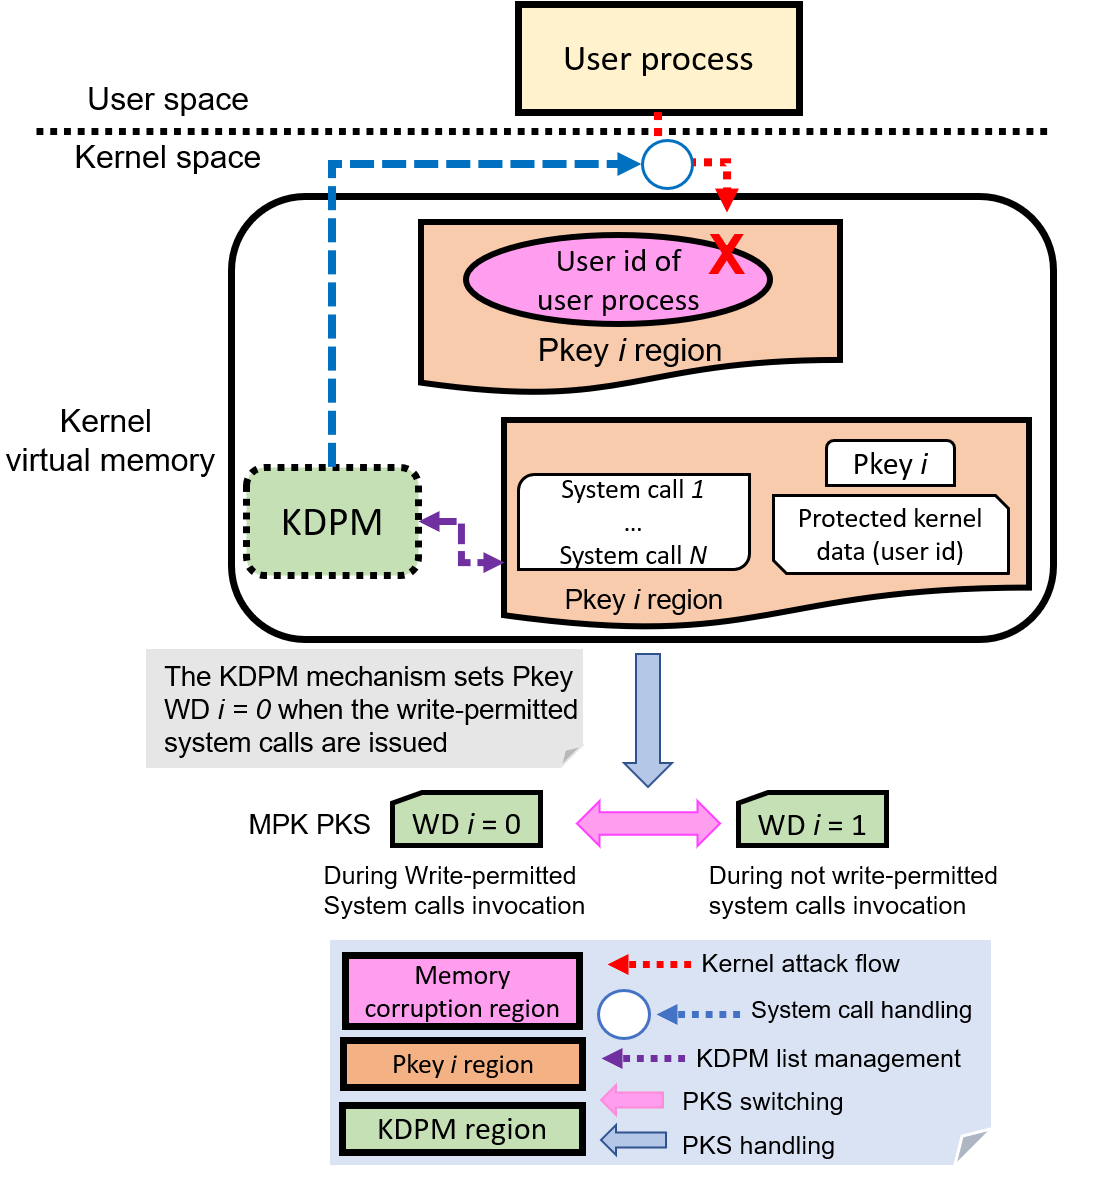
\includegraphics[bb=0 0 826 887, scale=.260]{./imgs/004_screenshot_2021-07-28_18.34.36.png}
  \end{center}
  % \vspace{-2.0ex}
  \caption{
    %
    % 提案するセキュリティ機構の実現方式1
    Implementation 1 of the KDPM
    %
  }
  % \vspace{-3.0ex}
 \label{fig:implementation1_overview}
\end{figure}

\begin{table}[t]
  \centering
    \caption{
      % 実現方式1における保護対象カーネルデータと書込み許可システムコール(参考文献 \cite{yamauchi21ijis} より抜粋)
      Protected kernel data and write-permitted system call of Implementation 1 
    }
\scalebox{1.00}{
%\hspace*{-5.0ex}  
\begin{tabular}{lc}
  %\hline
  \hline \noalign{\smallskip}
  \begin{tabular}{c}
    {\bf Item}
  \end{tabular}
  & 
  \begin{tabular}{c}  
  {\bf Description}
  \end{tabular}
  \\         
  \noalign{\smallskip}
  \hline
  \noalign{\smallskip}
  \multirow{2}{*}{Protected kernel data} & User ID (e.g., uid,euid,fsuid,suid)\\
                                         & Group ID (e.g., gid,egid,fsid,sgid)\\
  \multirow{2}{*}{Write-permitted system call}   & execve, setuid, setgid, setreuid, setregid\\
                                         & setresuid, setresgid, setfsuid, setfsgid\\         
  \hline
\end{tabular}
}
\label{tb:systemcall_list}
\end{table}


% \subsubsection{保護対象カーネルデータの書込み制御} \label{subsubsection:imp01_write_handling}
\subsubsection{Handling of Write Restrictions:} 

% 実現方式1において,書込み許可システムコールのリストに含めるシステムコールは,権
% 限情報の操作を行うシステムコールとし,\tabref{tb:systemcall_list}に示す.実現方
% 式1における, PKS Pkey を用いた保護対象カーネルデータの書込み制限の制御
% は,次の手順にて行う.
% The system calls to be included in the list of write permitted system calls in
% implementation method 1 shall be system calls that perform operations on
% authorization information. 

Implementation 1 admits the system calls that change the privileged
information (Figure \ref{tb:systemcall_list}). 
%
The process of controlling the write restrictions of the protected kernel data using Pkey is as follows:
% in implementation method 1 The following
% procedure is used.

% \begin{enumerate}[topsep=0pt]%\itemsep=-1.0ex \parskip=1.0ex  
\begin{enumerate}%[topsep=0pt]%\itemsep=-1.0ex \parskip=1.0ex  
%   \item ユーザプロセスによるシステムコール呼出しを捕捉.
\item The kernel identifies a system call invoked by a user process.
  
  
%   \item 書込み許可システムコールリストに含むシステムコール番号か判定.
\item The kernel determines if the system call number is included in the list of write-permitted system calls.

\begin{enumerate}%[topsep=0pt]%\itemsep=-1.0ex \parskip=1.0ex      
%   \item 書込み許可システムコールの場合:
%   PKSによる書込み制限制御を行い,保護対象カーネルデータを書込み許可に設定.
\item For write-permitted system calls: the kernel sets the protected kernel data with
the write-enable permission by the PKRS.
\end{enumerate}
  
% \item システムコールの実行を継続する.
% \item システムコールの終了後,
% PKSによる書込み制限制御を行い,保護対象カーネルデータを書込み制限に設定.
\item The execution of the system call is continued.
\item After the system call: the kernel restores the protected kernel data and
is set to the write-disable permission by the PKRS.
% writes restriction control 
% and 
% is performed

\end{enumerate}


% \subsection{実現方式2の個別処理}
\subsection{Implementation 2} \label{subsection:imp02_write_handling}

% 実現方式2の概要を図\ref{fig:implementation2_overview}に示す.実現方式2において
% は,書込み許可カーネルコードとして,セキュリティ機能の変更を伴うカーネルコード
% 実行時のみセキュリティ機能に関するカーネルデータの書込み制限を制御するため,
% LSMに関するカーネルデータの一覧,および書込み許可カーネルコードの一覧をリスト
% として管理する.
Figure \ref{fig:implementation2_overview} presents an overview of Implementation
2.
%
Implementation 2 adopts the write-permitted kernel code of the LSM and supports
the list of kernel data related to the LSM and that of the write-permitted
kernel codes.
% the kernel code for LSM is 
% In Scheme 2, the kernel code for LSM is the write-allowed kernel code.
%
Implementation 2 handles the write restrictions for the protected kernel data when
executing write-permitted kernel codes that change the access control policy and
access control decision.
%



% \subsubsection{保護対象カーネルデータ}
\subsubsection{Protected Kernel Data:}


\begin{figure}[t]
  \begin{center}
%    \hspace*{-5.0ex}
    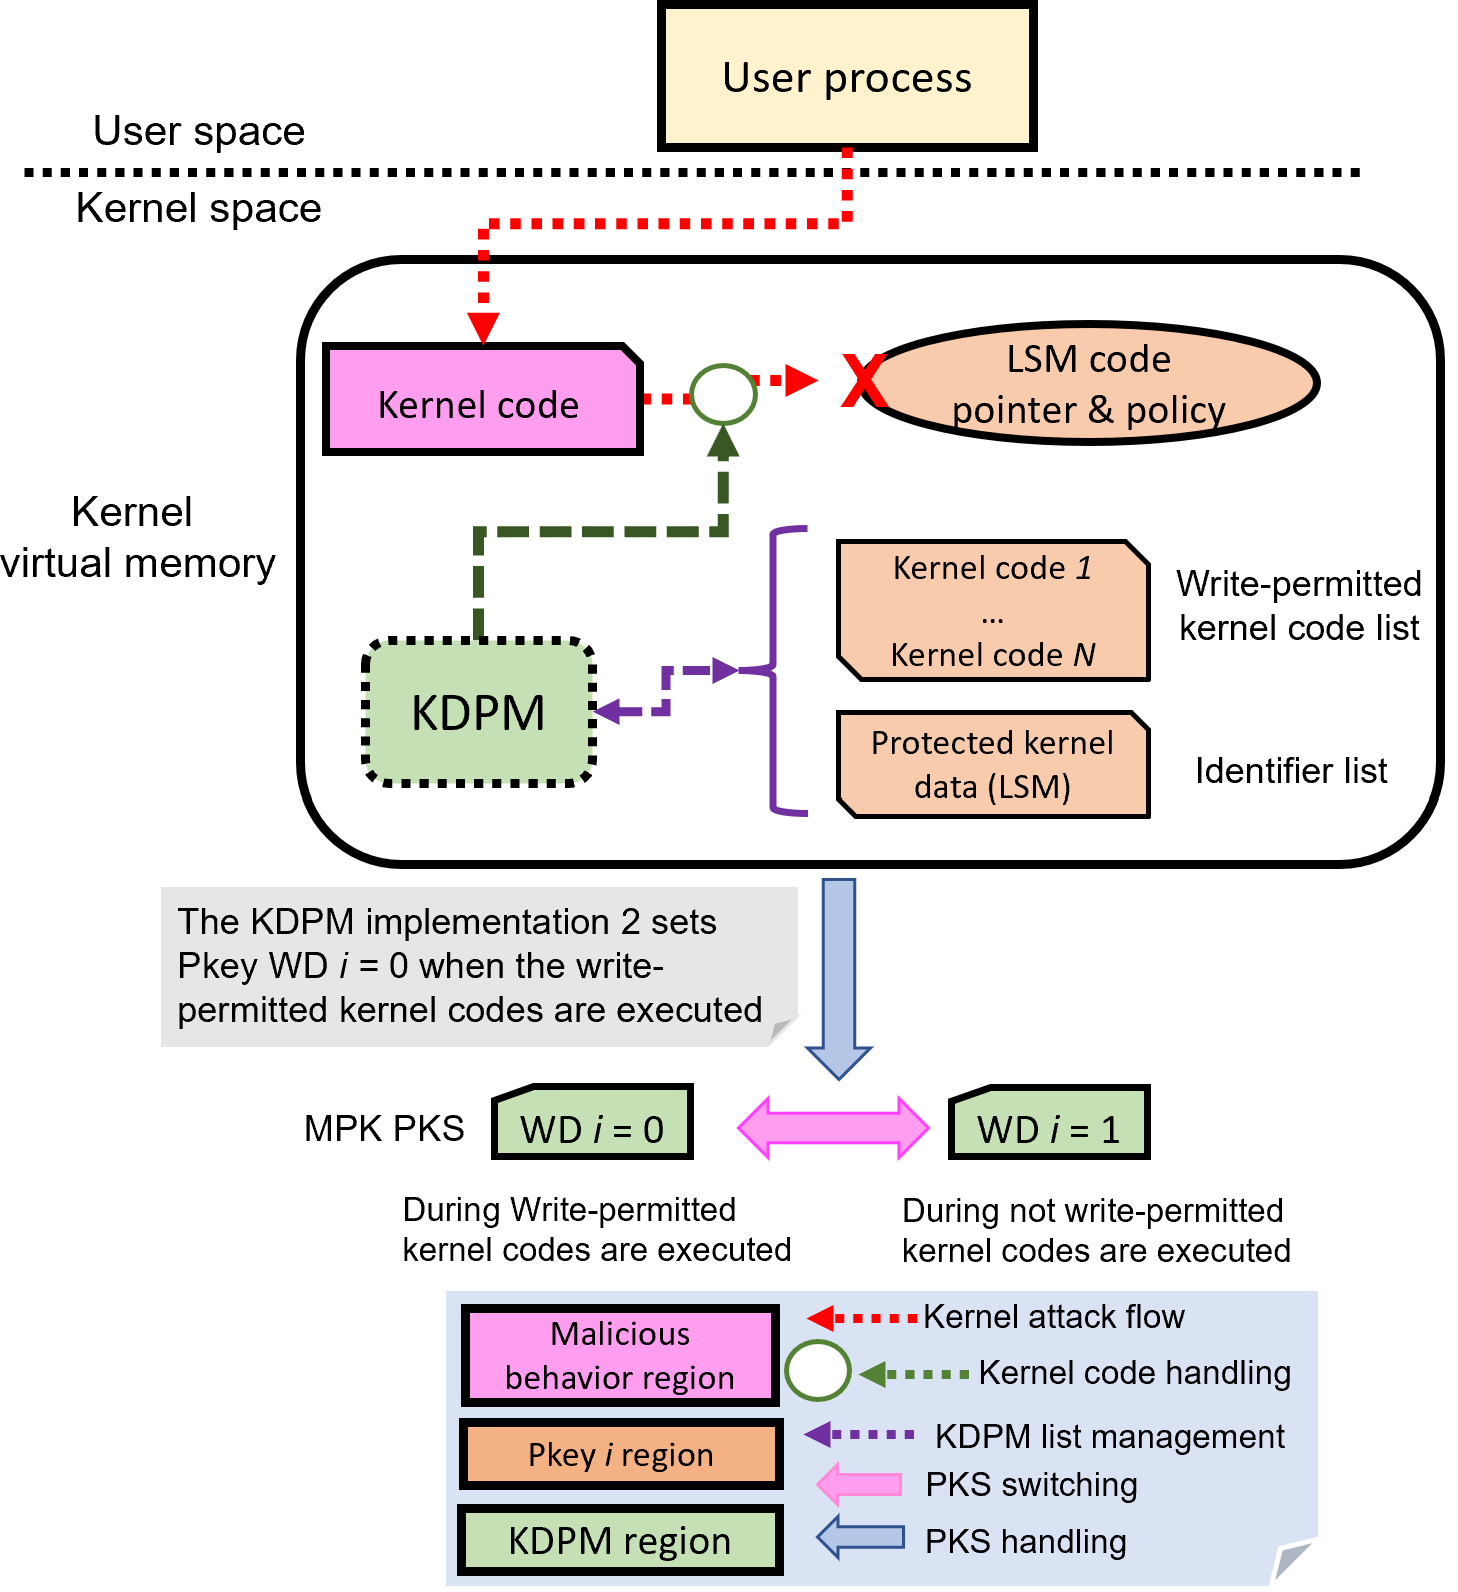
\includegraphics[bb=0 0 875 923, scale=.280]{./imgs/005_screen_shot_2022-01-10_180226.png}
  \end{center}
  % \vspace{-2.0ex}
  \caption{
    %
    % 提案するセキュリティ機構の実現方式2
    Implementation 2 of the KDPM
    %
  }
  % \vspace{-3.0ex}
 \label{fig:implementation2_overview}
\end{figure}


% 実現方式2において,保護対象とするカーネルデータは,\tabref{tb:kernel_code_list}
% に示すLSMに関連するカーネルデータの一部である関数ポインタを格納する変数,ならび
% にアクセス制御ポリシを格納する変数とるす.また,書込み許可カーネルコードのリスト
% についてもPKSを用いた書込み制限制御による保護対象とする.
Table \ref{tb:kernel_code_list} presents the kernel data to be protected in
Implementation 2. Additionally, \verb|selinux_hooks| is a variable that stores function
pointers that are part of the kernel data related to the LSM, and
\verb|selinux_state| is a variable that stores the access control policy. Furthermore,
the list of write-permitted kernel codes is protected by write restriction
control using the PKS.


\begin{table}[t]
  \centering
    \caption{
      % 実現方式2における保護対象カーネルデータと書込み許可カーネルコード.
      Protected kernel data and write-permitted kernel code of Implementation 2
    }
\scalebox{0.85}{
%\hspace*{-5.0ex}  
\begin{tabular}{lc}
  %\hline
  \hline \noalign{\smallskip}
  \begin{tabular}{c}
    {\bf Item}
  \end{tabular}
  & 
  \begin{tabular}{c}  
  {\bf Description}
  \end{tabular}
  \\         
  \noalign{\smallskip}
  \hline
  \noalign{\smallskip}
  \multirow{2}{*}{Protected kernel data} & Function pointer (e.g., selinux\_hooks)\\
                                         & Security policy (e.g., selinux\_state)\\
  \multirow{2}{*}{Write-permitted kernel code}   & Kernel functions in the selinux\_hooks\\
                                                 & avc\_init, avc\_insert, avc\_node\_delete, avc\_node\_replace\\         
  \hline
\end{tabular}
}
\label{tb:kernel_code_list}
\end{table}

% \subsubsection{保護対象カーネルデータの書込み制御} \label{subsubsection:imp02_write_handling}
\subsubsection{Handling of Write Restrictions:} 

% 実現方式2における保護対象カーネルデータのうち,LSMに関連するカーネルデータの関数
% ポインタを格納する変数,および書込み許可カーネルコード名リストは Linux カーネル
% の起動中に値が設定される.
% %
% 実現方式2においては,個々の値がカーネルデータに格納された直後にPKSによる書込み制
% 限対象とし,管理する.
% Among the kernel data to be protected in 
Implementation 2 stores the function pointer of the kernel data related to
the LSM, and the list of write-permitted kernel codes is set during the booting of the kernel.
% at the kernel booting.
%  to values during Linux kernel
% startup.
Table \ref{tb:kernel_code_list} also presents the kernel codes to be included in
the list of write-permitted kernel codes.

% In Implementation Scheme 2, each value is subject to write restriction by PKS
% immediately after it is stored in the kernel data, and is managed.

% %

% 実現方式2における書込み許可カーネルコードに対するPKSを用いた制限制御は次の手順にて行う.
The following procedure is used to control the restrictions on the write-permitted
kernel code using the PKS:
% in implementation method 2 

% %\begin{enumerate}
\begin{enumerate}[topsep=0pt]%\itemsep=-1.0ex \parskip=1.0ex  
%   %\item ユーザプロセスのコンテキストスイッチの発生を捕捉する.
%   \item 書込み許可カーネルコードにより,実現方式2のカーネルコードを呼出す.
\item The kernel invokes the kernel code of Implementation 2 during the execution of the write-permitted kernel code.
%  calls the kernel code of implementation method 2
  
%   %\item システムコール番号が権限変更許可リストに含まれるか判定.
%   \item 実現方式2のカーネルコードにて,書込み許可カーネルコードからの呼出しか判定.
\item The kernel code of Implementation 2 determines whether the caller belongs to a write-permitted kernel code.

% %  \begin{enumerate}
\begin{enumerate}[topsep=0pt]%\itemsep=-1.0ex \parskip=1.0ex      
%   \item 書込み許可カーネルコードの場合:PKSによる書込み制限制御を行い,保護対象カーネルデータを書込み許可に設定.
\item In the case of a write-permitted kernel code, the kernel performs write restriction control using the PKS to set the protected kernel data as write enabled.
%   \item 保護対象カーネルデータの書込み制限設定を検証するカーネルコードをタイマに登録,一定期間後に呼出すよう設定.
\item The kernel registers the write restriction of the protected kernel data in the timer and sets it to be called after a certain time.
% kernel code that verifies the write limit setting of the kernel data to be protected in the timer and set it to be called after a certain period of time.
      
\end{enumerate}
  
% \item 書込み許可カーネルコードの処理を継続.
\item The kernel continues processing the write-permitted kernel code.
% \item 書込み許可カーネルコードの終了前,実現方式2のカーネルコードを呼出し,
% PKSによる書込み制限制御を行い,保護対象カーネルデータを書込み制限に設定.
\item Before the end of the write-permitted kernel code, the kernel code of
Implementation 2 is called. The kernel performs write restriction using the PKS to set the
protected kernel data as write disabled.
% to be protected as write-limited.
% \item 書込み許可カーネルコードの処理を終了
\item The kernel finishes the processing of the write-permitted kernel code.

\end{enumerate}

% 書込み許可カーネルコードのリストに含めるカーネルコードは,
% \tabref{tb:kernel_code_list}のLSMの制御ポリシの操作を行うカーネルコードとする.

% 実現方式2において,タイマ登録される書込み制限設定を検証するカーネルコードでは,
% 書込み許可が意図せずに継続されることを防止する.
% %
% 書込み許可と制限を設定するカーネルコードの呼出し回数が一致しない場合,ならびに書
% 込み許可の継続時間が規定時間を超えた場合,強制的に書込み制限に設定する.
%
Implementation 2 verifies the write restriction setting using the timer to
prevent write as enable continued unintentionally.
% registered in 
%
% The implementation 2 is forced to set the write restriction.
% If 
Implementation 2 also checks the number of kernel code invocations to determine whether the
write restriction enabled and disabled are the same.
%
Further, Implementation 2 verifies whether the duration of write enable exceeds
the specified time.
%
% \reduline{ 
The timer is a complementary feature to prevent missing of the configuration of
  the PKS protection setting. 
% to prevent the miss configuration of PKS protection setting. 
%
This timer usually requires sufficient time to miss it between starting and
finishing the execution of the write-permitted kernel code.
% execution start and finish.}
%  are not match, 


% \subsubsection{読書き制限の管理と操作}

% 実現方式において,権限情報 Protection key {\it i}に対する読書き制限
% RD{\it i},およびWD{\it i}は PKS の読書き制限操作レジスタ
% \verb|IA32_PKRS MSR|を用いて管理する.
% %
% %\verb|IA32_PKRS MSR|はCPUのコア単位に備えつけられており,権限変更許可
% \verb|IA32_PKRS MSR|はCPUコア毎に備えており,権限変更許可システムコー
% ル,および通常システムコール捕捉時の権限情報 Protection keyの読書き制
% 限の操作は,次の手順にて行う.

% %\begin{enumerate}
% \begin{enumerate}[topsep=0pt]\itemsep=-1.0ex \parskip=1.0ex  
%   \item ユーザプロセスによるシステムコール呼出しを捕捉.
  
%   \item 権限変更許可リストに含むシステムコール番号か判定.
  
% %  \begin{enumerate}
% \begin{enumerate}[topsep=0pt]\itemsep=-1.0ex \parskip=1.0ex      
%   \item 権限変更許可システムコールの場合:Protection key {\it i}に対応
%     する \verb|IA32_PKRS MSR| の RD{\it i},WD{\it i} に 0 を書込む
%     権限情報カーネルデータの読書き許可に設定
    
%   \item 通常システムコールの場合:Protection key {\it i}に対応する
%     \verb|IA32_PKRS MSR| の RD{\it i}に0を書込み,WD{\it i} に 1 を書
%     込む.権限情報カーネルデータの読込みのみ許可,書込みは不許可に設定.
%   \end{enumerate}
  
% \item システムコールの実行を継続する.
% \end{enumerate}


% 権限変更許可リストに含めるシステムコールは,
% \tabref{tb:privilege_data_list}の権限情報カーネルデータの操作を行うシ
% ステムコールとし,\tabref{tb:systemcall_list}に示す.


% \subsubsection{権限情報カーネルデータの保護事例}

% 実現方式を用いた権限情報カーネルデータの保護事例を
% \figref{fig:sample_case}に示す.
% %
% ユーザプロセスを起動後,権限情報 Protection key 1を権限情報カーネルデー
% タに設定する.
% %
% ユーザプロセスの発行したシステムコールが権限変更許可リストに含まれてい
% る場合,カーネルにおいてシステムコールの実行中,読書き制限操作レジスタ
% \verb|IA32_PKRS MSR| の RD1 および WD1 を 0 とし,権限情報の読書き操作
% を許可する.
% %
% 一方,システムコールが権限変更許可リストに含まれていない場合,システム
% コールの実行中,読書き制限操作レジスタ \verb|IA32_PKRS MSR| の RD1 は
% 0,WD1 は 1 とし,権限情報の書込みは許可されない.
% %

% \begin{figure}[tb]
%   \begin{center}
%     \hspace*{-5.0ex}
%     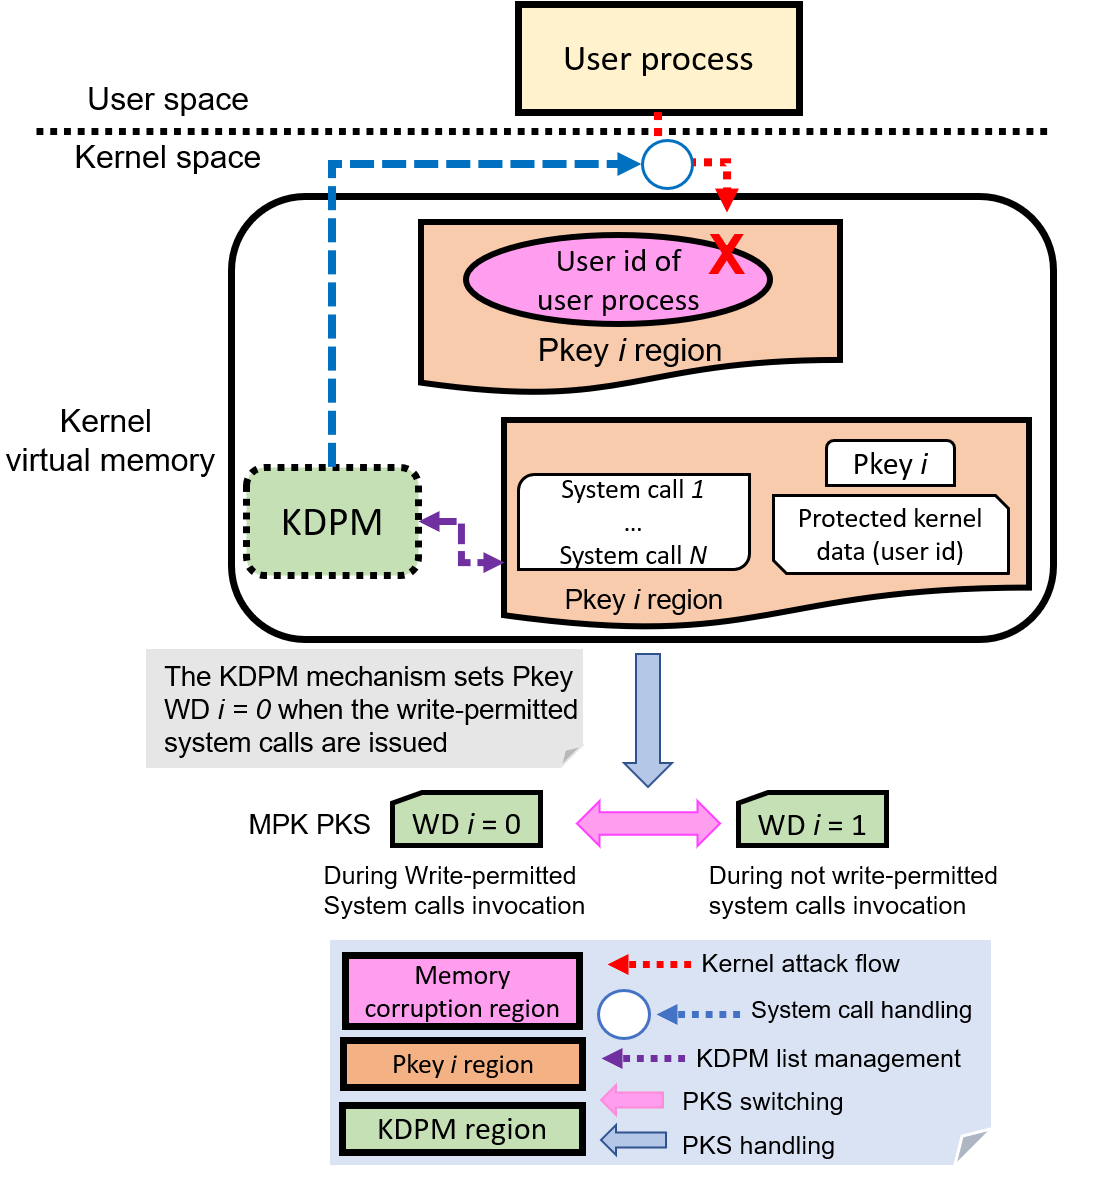
\includegraphics[bb=0 0 1033 887, scale=.265]{./imgs/004_screenshot_2021-07-28_18.34.36.png}
%   \end{center}
%   \vspace{-2.0ex}
%   \caption{
%     %
%     実現方式を適用した権限情報カーネルデータの保護
%     %
%   }
%   \vspace{-3.0ex}
%  \label{fig:sample_case}
% \end{figure}


%\subsubsection{プロファイル生成手順}
% \subsection{Profile Generation}
% vkTracer automatically generates a profile of the kernel vulnerability. 
% %
% Figure \ref{fig:approach_flow_overview} illustrates the steps of
% profile generation, which employs the trapping of the invocation of
% the kernel code and the identification of the virtual address ranges
% of the running kernel.
% This is achieved through the following steps:

% \begin{itemize}
% \item {\bf Step 1-1:}
%   The adversary executes the PoC code as a user process. vkTracer attaches to the adversary's user process and then registers the tracing target \verb|pid| for trapping.
  
% \item {\bf Step 1-2:}
%   The adversary's user process starts the kernel attack, which invokes the vulnerable kernel code by exploiting the kernel vulnerability.

% \item {\bf Step 1-3:} vkTracer determines whether the user process id
%   is the tracing target \verb|pid|, and then collects information on
%   the kernel code that is invoked by the adversary's user
%   process during each system call invocation.

% \item {\bf Step 1-4:}  vkTracer terminates the trapping of
%   the adversary's user process when the kernel is compromised through
%   the kernel vulnerability.

% \item {\bf Step 2-1:} vkTracer extracts the necessary kernel
%   information (e.g., invocation of kernel codes) from static and
%   dynamic kernel images to generate a profile of the kernel
%   vulnerability.


% \item {\bf Step 2-2A:} If the running kernel does not use KASLR, then vkTracer
%   creates a relationship among the kernel code, function name, and virtual
%   address ranges using the debug information of the kernel for the profile.

    
% \item {\bf Step 2-2B:} If the running kernel does use KASLR, then vkTracer
%   specifies whether the kernel image contains the kernel code as part
%   of the profile. The complement of the virtual address ranges is
%   identified for the profile at the kernel boot.
  
  
% \end{itemize}


% \subsection{Kernel Code Tracing}

% vkTracer uses the kernel tracing capabilities (e.g.,
% %
% \verb|bpftrace| and \verb|tracepoints|)
% %
% to associate the running kernel with the user process behavior.  The left
% side of Figure \ref{fig:tracing_implementation_overview} shows an
% overview of the tracing implementation and uses the following definitions.
% %% to attache the running kernel and user process behavior. The left side
% %% of Figure \ref{fig:tracing_implementation_overview} indicates the
% %% overview of tracing implementation.

% \begin{itemize}
% \item {\bf tracepoints}: This is a static embedded placement of a kernel that calls the tracing mechanism to record kernel processing.
%   %It is a static embedded placement of a kernel that calls the tracing mechanism
%   %to record the kernel processing.

% \item {\bf kprobes}:
%   This is a dynamically registered placement of a kernel that uses the symbol information of a function name for the kernel tracing capability.
  
%   %It is a dynamically registered placement of a kernel that
%   %uses the symbol information of a function name for kernel tracing capability.
%   %to calls an user defined enhanced Berkeley Packet Filter (eBPF) program 
% \end{itemize}

% The implementation of vkTracer employs the entire suite of kernel symbols and
% hooks the invocations of kernel code through \verb|kprobes|,
% %
% %The implementation of vkTracer employs the entire suite of kernel symbols and
% %hooks to the the invocations of kernel code thorough \verb|kprobes|.
% %
% whereas \verb|tracepoints| provides additional information about the kernel activity (i.e., system calls). 
% %
% %provides additional information of the kernel activity (i.e., system calls).
% %
% The implementation of vkTracer registers both tracing capabilities as
% a user-defined enhanced Berkeley Packet Filter (eBPF) program in the
% running kernel.
% %
% Therefore, vkTracer gathers the actual kernel code
% invocation history (e.g., function name list) from the target user
% process for the generation of the profile.

%% The implementation of vkTracer registers both tracing capabilities as user-defined enhanced Berkeley Packet Filter (eBPF) program into the running kernel.
%% %
%% Therefore, vkTracer gathers the actual kernel code invocation history (e.g., function name list) from the target user process for the generation of the profile. 
  


% \subsection{Virtual Address Range Identification}
% vkTracer analyzes the static and dynamic kernel images to identify the virtual
% address ranges for each kernel code for profile generation.
% %
% %vkTracer analyzes the static kernel image and the dynamic kernel image to identify the virtual address ranges for each kernel code for the profile generation.
% %
% Figure \ref{fig:tracing_implementation_overview} shows an overview of
% the virtual address identification implementation, which includes the following analyses:
% %indicates the overview of virtual address identification implementation.

% \begin{itemize}
% \item {\bf Static analysis of the kernel}:
%   %
%   vkTracer employs several sections of the Linux kernel. These are DWARF and
%   symbol information include \verb|.debug_info| and \verb|.text|, which contain
%   the kernel code and virtual address information.
  
%   %% vkTracer employs several sections of the
%   %% Linux kernel.  These are debug with attribute record format (DWARF)
%   %% is 
%   %% contains the kernel code and virtual address information.
% % \item 静的な仮想アドレス特定手段:KASLR有無に関わらず利用.カーネルの
%    %  DWARF情報として,カーネルデバッグに必要な情報として,\verb|.debug_info|
% %   \verb|.debug_info| セクションに格納されるDWARF(Debug With Attribute
% %     Record Format)情報,ならびにカーネルコードに関する \verb|.text|セク
% %   ションの情報を利用して仮想アドレス範囲を特定

% \item {\bf Dynamic analysis of the kernel}: vkTracer dynamically identifies the
%   virtual address range of the kernel code using the function name from
%   \verb|kprobes| and \verb|tracepoints| of the eBPF program.
%   %
%   Then, vkTracer prepares the Linux kernel module (LKM) that
%   requires the modified Linux kernel to employ \verb|EXPORT_SYMBOL| for
%   almost all kernel functions. It allows the LKM of vkTracer to
%   directly access the virtual address of the specified kernel function at
%   the kernel layer.
%   %vkTracer directory identifies the virtual address range of kernel code using the function name at the kernel layer.
% %}
% % \item 動的な仮想アドレス特定手段:KASLR有効時に利用,カーネルの起動時
% %   にカーネルコードを直接参照し,仮想アドレス範囲を特定
%  \end{itemize}

% The DWARF files contain multiple records of a program for debugging purposes.
% vkTracer parses the entirety of the records, and creates a relationship among
% the traced kernel code, virtual address range, and function name for the profile
% generation.
% %
% Table \ref{tb:dwarf_information} lists the DWARF information for the
% static analysis of the kernel. However, if the kernel uses
% KASLR, which performs a randomization of the virtual address range of
% the kernel code at each kernel boot, then vkTracer depends on a dynamic
% analysis of the kernel image to avoid infection from KASLR.


% \begin{table}[h]
%  \centering

% \caption{
% %
%   %  Portability consideration of MKM mechanism for OSes ($\checkmark$ is supported; $\triangle$ is partially supported).
%   DWARF information for profile ($\checkmark$ is adopted).
% %
% }
% %\vspace{-0.5ex}  
% \scalebox{1.00}{
% %  \begin{tabular}{c|cc}
% \begin{tabular}{llc}    
% %\hline
% \hline
% \noalign{\smallskip}
% %\begin{tabular}{c}
% %  {\bf Feature}
% %\end{tabular}
% \begin{tabular}{c}
%   {\bf Item}  
% \end{tabular}
% &
% \begin{tabular}{c}
%   {\bf Description}  
% \end{tabular}
% &
% \begin{tabular}{c}
%   {\bf Profile}
% \end{tabular}
% \\
% \noalign{\smallskip}
% \hline
% \noalign{\smallskip}
% DW\_AT\_name         & Function name                      & $\checkmark$ \\
% %DW\_AT\_decl\_file   & Function definition file name      & $\bullet$ \\
% %DW\_AT\_decl\_line   & Function definition line number    & $\bullet$ \\
% %DW\_AT\_type         & Return value type of function      & $\bullet$ \\
% DW\_AT\_low\_pc      & Lower virtual address of function  & $\checkmark$ \\ 
% DW\_AT\_high\_pc     & Higher virtual address of function & $\checkmark$ \\ 
% \hline
% \end{tabular}
% }
% \label{tb:dwarf_information}
% %\vspace{-1.0ex}  
% \end{table}



% \subsection{Termination Condition} \label{subsubsection:tracing_condition}

% vkTracer implements the following conditions for tracing completion:
% %  vkTracer implements the condition of tracing completion as following.  %}

% \begin{itemize}%\itemsep=-1.0ex \parskip=1.0ex

% \item {\bf Privilege escalation}: The adversary's user process
%   forcibly modifies its credential information (e.g., \verb|UID| is
%   \verb|0|) from normal privilege to administrator privilege.
% %  The adversary's user process forcibly modifies its credential
% %  information to the administrator privilege from the normal privilege.

% \item {\bf DoS}: The adversary's user process forcibly suspends the running
%   kernel after exploiting the kernel vulnerability. At this point, it will be
%   difficult to continue tracing the user process and kernel. Therefore, vkTracer
%   writes the history of the vulnerable kernel code's invocation to the disk
%   or sends these data to a remote server.

%   %% The adversary's user process forcibly suspend the running kernel
%   %% after the exploiting of kernel vulnerability.  It is difficult to
%   %% continue the tracing of user process and kernel, vkTracer writes the
%   %% history of vulnerable kernel code invocation to the disk or send
%   %% these to the remote server.

% \end{itemize}


% \subsection{Case Study}

% \subsubsection{User process tracing and kernel code identification}
% %\subsubsection{ユーザプロセスの追跡例}

% A case study was performed on the user process tracing and virtual address range
% for kernel code identification based on the profile of a specific kernel code
% (\verb|vfs_write|) using vkTracer.
% %
% As a demonstration of the tracing condition (in Section \ref{subsubsection:tracing_condition}),
% %
% Figure \ref{fig:tracing_sample_case} shows that the user process
% invokes a write system call and then switches its privilege from that
% of a user account to an administrator level.
% %
% vkTracer attaches to the user process, catches the invocation of
% the \verb|vfs_write| kernel code, and then finishes the tracing when
% the privilege of the user process becomes that of the administrator.
% % account.
% %
% Subsequently, vkTracer identifies the virtual address range of the
% \verb|vfs_write| kernel code, which is \verb|ffffffff811b8cd0| to
% \verb|ffffffff811b8e64| for the profile of \verb|vfs_write|.

% \begin{figure}[t]
%   \centering
%   \includegraphics[bb=0 0 541 457, scale=.275]{./imgs/A01X_04_screenshot_2021-05-26_4_38_28.png}

%     %  \vspace{-4.5ex}  
%   \caption{
%     %
%     Case study of tracing and kernel code identification
%     %
%   }
%   \label{fig:tracing_sample_case}
% %\vspace{-5.0ex}        
% \end{figure}



%% As case study of user process tracing and virtual address range of kernel code identification
%% as the profile of specific kernel code (e.g., \verb|vfs_write|) on vkTracer.
%% %
%% Figure \ref{fig:tracing_sample_case} shows that the user process invokes
%% %
%% \verb|write|
%% system call, then switches its privilege to administrator level from user account
%% for the demonstration of tracing condition (section \ref{subsubsection:tracing_condition}).
%% %
%% vkTracer attaches the user process and catches the invocation of 
%% %
%% \verb|vfs_write|
%% %
%% kernel code, then finishes the tracing when the privilege of the user
%% process becomes that of administrator account. After that, vkTracer
%% identifies the virtual address range of
%% %
%% \verb|vfs_write|
%% %
%% kernel code which is
%% %
%% \verb|ffffffff811b8cd0| to \verb|ffffffff811b8e64|
%% %
%% for the profile of \verb|vfs_write|.


%% \subsection{Restriction Implementation}


%% \blueuline{
%% The implementations of restriction of KPRM on a Linux kernel with x86\_64 CPU
%% architecture.
%% %
%% Linux with the restriction of KPRM manages the kernel page table that
%% controls the visible kernel pages for an adversary's user process.
%% }

%% Table \ref{tb:consideration_implementation} illustrates \blueuline{the
%% restriction of KPRM implementations, comparing their different
%% characteristics and effects.}
%% %
%% Figures \ref{fig:approach_implementation_1} shows that \blueuline{the restriction of
%% KPRM implementation 1 can prevent invocation of vulnerable kernel code and
%% protect kernel data.}
%% \blueuline{
%% It controls the references of restricted kernel pages on the additional
%% kernel address space of kernel page table for the adversary's user
%% process.}
%% %
%% Figure \ref{fig:approach_implementation_2} shows that \blueuline{the restriction of
%% KPRM implementation 2 can prevent kernel data memory corruption. It
%% requires complex handling for the references of restricted kernel pages
%% on the shared kernel address space of one kernel page table.}

%% \begin{table}[h]
%%  \centering

%% \caption{
%% %
%%     Implementations of KPRM ($\circ$ is covered; $\bullet$ is non-covered;).
%% %
%% }
%% %\vspace{-1.0ex}  
%% \scalebox{1.0}{
%% %  \begin{tabular}{c|cc}
%% \begin{tabular}{ccc}    
%% %\hline
%% \hline
%% %\noalign{\smallskip}
%% %\begin{tabular}{c}
%% %  {\bf Feature}
%% %\end{tabular}
%% {\bf Item}  & {\bf Implementation 1} & {\bf Implementation 2}\\
%% %\noalign{\smallskip}
%% \hline
%% %\noalign{\smallskip}
%% Kernel data protection         & $\circ$      & $\circ$  \\
%% Kernel code restriction         & $\circ$      & $\bullet$ \\
%% Stability effect                & Low          & High \\
%% Performance effect              & High         & Low \\
%% \hline
%% \end{tabular}
%% }
%% \label{tb:consideration_implementation}
%% %\vspace{-3.0ex}  
%% \end{table}


%% \begin{figure*}[t]
%%   \centering    
%%   \hspace*{-10.0ex}    
%%     \includegraphics[bb=0 0 1771 999, scale=.245]{./imgs/004_screen_shot_2019-08-04_12.55.50.png}
%% %  \vspace{-1.0ex}
%%   \caption{
%%     %
%%     Implementation 1 of kernel page restriction mechanism
%%     %
%%   }
  
%% %  \vspace{-1.0ex}  
%%   \label{fig:approach_implementation_1}
%% %  \vspace{-1.0ex}
%% \end{figure*}



%% \begin{figure*}[t]
%%   \centering    
%%   \hspace*{-10.0ex}    
%%     \includegraphics[bb=0 0 1770 996, scale=.245]{./imgs/005_screen_shot_2019-08-04_13.49.13.png}
%% %  \vspace{-1.0ex}
%%   \caption{
%%     %
%%     Implementation 2 of kernel page restriction mechanism
%%     %
%%   }
  
%%   %\vspace{-1.0ex}  
%%   \label{fig:approach_implementation_2}
%% %  \vspace{-1.0ex}
%% \end{figure*}
 

%% \subsubsection{Restricted Kernel Page Management}

%% Linux with \blueuline{both the implementations of the KPRM handle}
%% benign identification \verb|benign| flag on the struct
%% \verb|task_struct| to user process.
%% %
%% \blueuline{the restriction of KPRM} enables \verb|benign| flag to
%% refer application binary's absolute path within the benign user
%% process list \verb|benign_user_process_list|.
%% This list is manually created in the kernel source code.
%% \reduline{Additionally, the administrator modifies} \verb|benign|
%% \reduline{flag management via} \verb|/proc/pid/kprm|.
%% %
%% %Linux with KPRM
%% \blueuline{The restriction of KPRM} also manages the restricted kernel
%% page list \verb|restricted_page_list| that stores the restricted
%% kernel page information including \reduline{the list of kernel data
%%   and virtual address and the list of kernel code, the virtual
%%   address, and function name from profiles of kernel vulnerability.}
%% %
%% %A virtual address is related to the kernel code or kernel data.
%% %


%% \subsubsection{Implementation 1}
%% %
%% \blueuline{The restriction of KPRM implementation 1
%%   adopts an additional kernel page table with the Linux kernel page table
%%   structure.} 
%% %
%% Figures \ref{fig:approach_implementation_1} \blueuline{indicates that
%%   the implementation 1 of KPRM kernel creates the kernel address space
%%   of the page table for the kernel and it is restricted to system
%%   calls for the user process.}
%% %
%% The additional kernel page table is the variable \verb|kprm| of
%% \verb|mm_strct| on the struct \verb|task_struct|.

%% The additional kernel page table duplicates the initial value
%% \verb|pgd| of \verb|init_mm| to \verb|kprm| for the user process
%% creation.
%% %
%% During the running of the kernel, the KPRM kernel prepares
%% the PCID of TLB and then writes \verb|kprm| in \verb|current| to the
%% CR3 register for system call invocation.
%% %
%% KPRM also applies the timing of restricted kernel page handling.

%% The Linux kernel executes a task under the kernel address space
%% constructed from variable \verb|pgd| of \verb|current| when the kernel
%% receives an asynchronous interruption.
%% %
%% To overcome the issue of interruption, implementation 1 of KPRM kernel
%% switches to the kernel address space from the additional kernel
%% address space \verb|kprm| of \verb|current|.
%% %
%% This requires the writing of the CR3 register with the kernel page
%% tables as the variable \verb|pgd| of \verb|current| with PCID of TLB.


%% \subsubsection{Implementation 2}
%% \blueuline{The restriction of KPRM implementation 2
%%  adopts the directory management of the original kernel page table}
%% (Figures \ref{fig:approach_implementation_2}).
%% %
%% The KPRM kernel uses the variable \verb|pgd| of \verb|current| at the
%% system call invocation for the timing of restricted kernel page
%% handling.

%% The KPRM kernel directory modifies the original kernel page table,
%% which leads to unstable kernel behavior during interruption
%% processing.
%% %
%% For handling an interruption, implementation 2 of KPRM kernel affixes
%% the restricted kernel page references to the original kernel page
%% table \reduline{for kernel tasks exectuion.}

%% \subsubsection{Page Fault}
%% \blueuline{
%% During the user processoth on the Linux kernel with both implementations of KPRM,}
%% %the implementations of the KPRM
%% %Both the implementations of the KPRM
%% %
%% Linux kernels catch the page fault with the \verb|do_page_fault| or
%% the \verb|do_double_fault| function.
%% %
%% These functions indicate the virtual address of the cause of the page
%% fault.
%% %
%% \blueuline{
%%   Subsequently, the restriction of KPRM kernel inspects the detail of page fault that whether 
%%   virtual address is available for the user process.}
%% %
%% It further determines the access decision and maps the restricted
%% kernel page to the current kernel page table when the user process is
%% valid. Otherwise, it uses \verb|force_sig_info| to send SIGKILL to the
%% user process \blueuline{for the forcibly termination.}


%% \subsubsection{Restricted Kernel Page Handling}

%% \blueuline{
%%   The restricted kernel page handling is the common process for both
%%   implementations of KPRM.
%%   The KPRM kernel automatically adopts the hadling for the adversary's user process.
%% }
%% %
%% \blueuline{The handling timing is hardcoded into the KPRM kernel that
%%   adopts the handling steps before system call invocation in the}
%% %
%% \verb|entry_SYSCALL_64| function.

%% The handling mechanism identifies the page number from the virtual
%% address and subsequently unmaps the \reduline{reference of} restricted
%% kernel page from the target kernel page table with the
%% \verb|remove_pagetable| function.
%% %
%% The restricted kernel page is also unmapped from the direct
%% mapping region.
%% %
%% \blueuline{
%% Additionally, KPRM kernel manages the page fault and trap handling related to
%% a restricted kernel page.
%% }

%% Figure \ref{fig:approach_attack_case_01} shows the handling mechanism
%% for an adversary process.
%% %
%% The restricted kernel page handling process is described below.


%% \begin{figure*}[t]
%% %  \begin{center}
%%   \centering    
%%   \hspace*{-4.0ex}        
%%     \includegraphics[bb=0 0 1759 976, scale=.250]{./imgs/003X_screen_shot_2019-08-04_16.52.28.png}
%% %  \end{center}
%% %  \vspace{-1.0ex}
%%   \caption{
%%     %
%%     KPRM for the adversary's user process    
%%     %
%%   }
%% %  \vspace{-2.0ex}  
%%   \label{fig:approach_attack_case_01}
%% %  \vspace{-2.0ex}
%% \end{figure*}




%% %\vspace{-1.0ex}    
%% %\begin{itemize}\itemsep=-1.0ex \parskip=1.0ex
%% \begin{enumerate} %\itemsep=-1.0ex \parskip=1.0ex
%%   %
%% \item \reduline{vkTracer preprares the profiles of
%%   kernel vulnerability for the handling process (section \ref{subsection:tracing_implementation}).}
  
%%   \item KPRM \blueuline{kernel} creates and stores restricted kernel
%%     pages to the restricted kernel page list
%%     and the benign user process list at kernel booting.

%%     \begin{enumerate}
%%     \item  \reduline{KPRM kernel registers the virutal address of kernel codes
%%       into the restricted kernel page list from the profiles of kernel vulnerability.
%%       Additionally, KPRM kernel also registers the virtual address of kernel doata
%%       into the restricted kernel page list from the list of protected kernel data.}
%%     \end{enumerate}
    
%%     %
%%   \item An adversary's user process starts the system call execution,
%%     following which the KPRM kernel traps the system call routing and moves
%%     to KPRM kernel processing.
%%     %
%%   \item
%%     KPRM kernel determines adversary's user process identifies with
%%     \verb|benign| flag is off, and then KPRM kernel restores the restricted
%%     kernel pages from the restricted kernel page list and subsequently
%%     unmaps all of \blueuline{their references of kernel page} in the
%%     kernel page table.
%%     %
%%   \item
%%     The system call is invoked along with access to the kernel code of the system call routine,
%%     following which the kernel issues the page fault and KPRM kernel traps the page fault.
%%     %
%%   \item
%%     KPRM kernel identifies the virtual address of the page fault that
%%     indicates the virtual address of kernel code is on the restricted
%%     kernel page.
%%     \begin{enumerate}
%%     \item  In case of an invalid accesses of the restricted kernel page,
%%       KPRM kernel denies access from the user process.
%%         %
%%     \item If the access is valid, KPRM kernel maps the reference of
%%       restricted kernel page of the kernel code  to the kernel page table
%%       for the user process to continue.
%%     \end{enumerate}
%%     %
%%   \item    
%%     The system call routine's kernel code accesses kernel data; then,
%%     the kernel also issues the page fault, and KPRM kernel traps the page
%%     fault.
%%     %
%%   \item KPRM kernel identifies the virtual address of the page fault that indicates
%%     the virtual address of kernel data is on the restricted kernel page.
%%     %
%%     \begin{enumerate}      
%%     \item In case of an invalid access of kernel data on the
%%       restricted kernel page, KPRM kernel denies access from the user
%%       process.
%%         %
%%     \item If the access is valid, KPRM kernel maps the restricted kernel page of kernel data
%%       to the kernel page table for the user process to continue.
%%     \end{enumerate}        
%%   \item If KPRM kernel determines an adversary's process, access is not
%%     allowed on the restricted kernel page, and KPRM kernel sends a signal to
%%     the user process.
%% \end{enumerate}  
%% %\vspace{-1.0ex}



%% %{\bf Vulnerable Kernel Code Invocation and Memory Corruption:}
%% \subsubsection{Vulnerable Kernel Code Invocation and Memory Corruption}
%% %
%% \blueuline{
%%   As a case study of kernel memory corruption exploits kernel vulnerability,
%% }
%% Figure \ref{fig:approach_actual_attack_case_01} shows that
%% \blueuline{the adversary's user process employs}
%% CVE-2017-16995 \cite{CVE-2017-16995} PoC code invokes the vulnerable
%% kernel code at the eBPF system call.
%% %
%% The vulnerable kernel code is the \verb|map_update_elem| function of
%% \verb|kernel/bpf/syscall.c|.
%% %
%% \blueuline{
%%   The adversary's user process tries to invoke the vulnerable kernel code
%%   to modify the virtual address of the privilege information of kernel data
%%   on the kernel address space. After the success of privilege escalation, the
%%   adversary's user process executes the shell with administrator privileges.
%% }  

%% To prevent such attacks, implementation 1 of the KPRM kernel specifies
%% the vulnerable kernel code as \verb|map_update_elem| function to the
%% restricted kernel page. Then, the adversary's user process cannot
%% invoke the vulnerable kernel code. 
%% %
%% \blueuline{
%% Additionally, both implementations of the KPRM kernel specify kernel
%% data (e.g., privilege information) to the restricted kernel page. The
%% adversary's user process of the PoC code cannot modify the restricted
%% kernel page.}
%% %
%% Next, a page fault of the restricted kernel pages occurs.
%% %
%% Both the implementations of the KPRM kernel can catch this page fault to
%% determine whether to send SIGKILL to the attack process in the page
%% fault handler.

%% \begin{figure*}[t]
%% %  \begin{center}
%%   \centering    
%%   \hspace*{-2.0ex}        
%%     \includegraphics[bb=0 0 1770 964, scale=.260]{./imgs/006_screen_shot_2019-08-07_15.54.13.png}
%% %  \end{center}
%% %  \vspace{-1.0ex}
%%   \caption{
%%     %
%%     Handling of restricted kernel page reference for the actual kernel vulnerability
%%     %
%%   }
%% %  \vspace{-2.0ex}  
%%   \label{fig:approach_actual_attack_case_01}
%% %  \vspace{-2.0ex}
%% \end{figure*}

%\subsection{Tracing Implementation} \label{subsection:tracing_implementation}

%% 提案手法の実現環境は x86\_64 CPUアーキテクチャの Linux を想定し,特定
%% のユーザプロセスを指定した際にカーネルコード呼出しの追跡ならびにカーネ
%% ルコードと仮想アドレス範囲の特定を行う実現方式を考案した.
%
%, as follows:
%In this study, the implementation of vkTracer is implemented on Linux for the
%x86\_64 CPU architecture.
%% indicates the steps of profile
%% generation that employs the trapping of the invocation of kernel code
%% and the identification of the virtual address ranges of the running
%% kernel as following:
%% \begin{itemize}
%% \item 特権奪取:攻撃を行うユーザプロセスの実行前後において,権限情報の
%%   通常ユーザから特権ユーザへの変化を攻撃成功とみなす.

%% \item DoS:攻撃を行うユーザプロセスの実行中にカーネルが停止した場合,
%%   攻撃成功とみなす.カーネルが停止する場合,カーネルコードの呼出し履歴
%%   の取得が困難となることから,永続性のある記録媒体へのカーネルコードの
%%   呼出毎の保存,またはリモートの計算機へのログ出力を行う.

%% \end{itemize}

%\reduline{vkTracer finishes the trapping of the PoC
%  code as the user process, vkTracer starts to generate a
%  profile of kernel vulnerability from the necessary information of
%  tracing result.}% in \ref{subsection:attack_scenario}. }

% \begin{figure*}[t]
%   \centering
%   %\hspace*{-8.0ex}  
%   \includegraphics[bb=0 0 1103 608, scale=.390]{./imgs/A01X_03_screenshot_2021-05-26_5_25_02.png}
%       %  \vspace{-4.5ex}  
%   \caption{
%     %
%     Implementation of profile generation
%     %
%   }
%   \label{fig:tracing_implementation_overview}
% %\vspace{-5.0ex}        
% \end{figure*}



%  The adversary executes the PoC code as the user process. vkTracer
%  attaches the adversary's user process, then registers tracing target \verb|pid| for the trapping.


  %The adversary's user process starts the kernel attack that
  %invokes the vulnerable kernel code through exploiting the kernel vulnerability.

  %% vkTracer determines whether the user process id is
  %% the tracing target \verb|pid|, then collects the kernel code information which is
  %% invoked by the adversary's user process during each the system call invocation.

  %% vkTracer extracts the necessary
  %% kernel information (e.g., the invocation of kernel codes) from the
  %% static and dynamic kernel image to generate the profile of kernel
  %% vulnerability.

  % KASLR randomized the virtual address ranges of the kernel code for each kernel boot. 
  
  %% vkTracer creates the relationship between the kernel code ,
  %% function name, and virtual address ranges using the debug information
  %% of the kernel for the profile when the running kernel does not adopt
  %% KASLR that randomizes virtual address ranges of kernel code for each
  %% kernel boot.
  
  %% If the running kernel adopts KASLR, vkTracer specifies
  %% that whether the kernel image contains the kernel code as the part of
  %% profile. The complement of virtual address ranges is identified for
  %% the profile at the kernel boot.
  
  %that KASLR randomizes virtual address range of kernel code for each kernel boot.%% The dwarf information contains multiple records of a program for debugging purposes. vkTracer parses the whole of records, then makes the relationship between the traced kernel code, virtual address range, function name for the profile generation.
%% %
%% Table \ref{tb:dwarf_information} shows the list of dwarf information
%% for static analysis of the kernel.
%% %  
%% In addition, due to the randomization of the virtual address range of kernel code at each KASLR enable kernel boot, vkTracer depends on the dynamic analysis of the kernel image to avoid the infection of KASLR.

%% 実現方式において,追跡対象のユーザプロセスを動作させ取得したカーネル関
%% 数名一覧から仮想アドレス範囲の特定は,以下の静的な仮想アドレス特定手段
%% ならびに動的な仮想アドレス特定手段により行う.両方の手段を利用するかは
%% カーネルの仮想空間におけるカーネルコードの位置を起動毎に変化させる
%% KASLRの有無に依存する.

%% \begin{itemize}
%% \item 静的な仮想アドレス特定手段:KASLR有無に関わらず利用.カーネルの
%%   %  DWARF情報として,カーネルデバッグに必要な情報として,\verb|.debug_info|
%%   \verb|.debug_info| セクションに格納されるDWARF(Debug With Attribute
%%     Record Format)情報,ならびにカーネルコードに関する \verb|.text|セク
%%   ションの情報を利用して仮想アドレス範囲を特定
  
%% \item 動的な仮想アドレス特定手段:KASLR有効時に利用,カーネルの起動時
%%   にカーネルコードを直接参照し,仮想アドレス範囲を特定
%% \end{itemize}

%% 静的な仮想アドレス特定手段にて用いるDWARF情報の値を表
%% \ref{tb:dwarf_information}に示す.DWARF情報を利用することで,仮想アド
%% レス範囲,定義ファイル,定義位置,関数の型,引数の数,ならびに引数の型
%% 等を特定することが可能である.

%% 追跡対象のユーザプロセスを実行した際,\ref{subsection:design} 節で示し
%% た一連の処理により,カーネルにおいてユーザプロセスから呼び出されたカー
%% ネルコードが列挙され,最終的にカーネルコードに対応する仮想アドレス範囲
%% の一覧が得られる.カーネルへの攻撃に紐づくカーネルコードかの判断は,カー
%% ネル脆弱性を利用した攻撃の成功可否を判定して行う.
%% %攻撃の成功可否を判定することが必要である.
%\reduline{
%
%  when
%the user process completes the attacking scenario (in section
%\ref{subsection:attack_scenario}) 
%% 提案手法においては,カーネル脆弱性を介して攻撃可能なPoC コードを実行す
%% る際に,以下のカーネル脆弱性毎の攻撃成功可否基準に従い,攻撃の有効性を
%% 判定する.
%% %攻撃成功時には基づいてカーネル脆弱性および関連するカーネルコードを特定する.

%% %,カーネルコードの推測が可能だと考えているが,CVE,PoCコー
%% %ド,ならびにカーネルのソースコード修正履歴を参照しながら特定する必要が
%% %ある.
